\section{Logarithms}\label{sec:Logarithms}
Recall the \ifont{three kinds} of exponential functions $f(x)=a^x$ depending on whether $0<a<1$, $a=1$ or $a>1$:
$$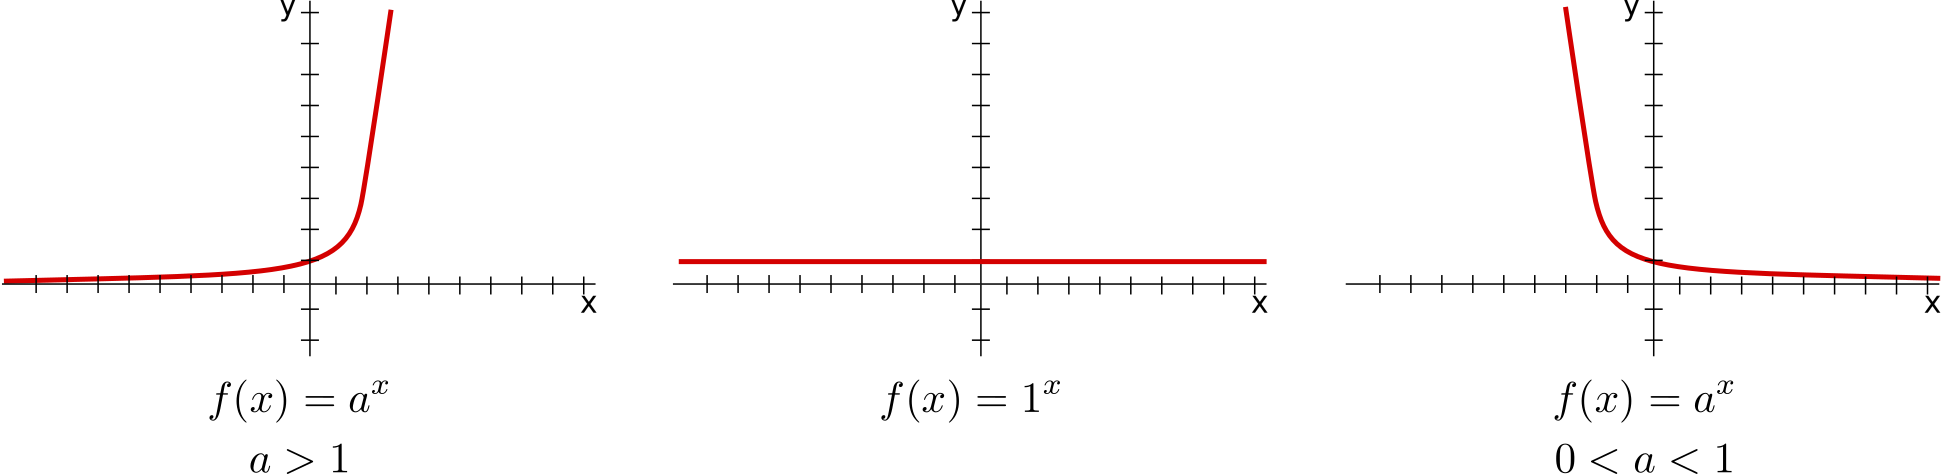
\includegraphics[width=6.5in]{images/exp3}$$
So long as $a\neq 1$, the function $f(x)=a^x$ satisfies the horizontal line test and therefore has an inverse.
We call the \ifont{inverse of $a^x$} the \dfont{logarithmic function with base a} and denote it by $\log_a$.
In particular,
$$\log_a x=y\iff a^y=x.$$
The \ifont{cancellation formulas} for logs are:
$$\log_a(a^x)=x,\mbox{\quad for every $x\in\R$},$$
$$a^{\log_a(x)}=x,\mbox{\quad for every $x>0$}.$$
Since the function $f(x)=a^x$ for $a\neq 1$ has domain $\mathbb{R}$ and range $(0,\infty)$, 
the logarithmic function has domain $(0,\infty)$ and range $\mathbb{R}$.
For the most part, we only focus on logarithms with a base larger than 
$1$ (i.e., $a>1$) as these are the most important.
$$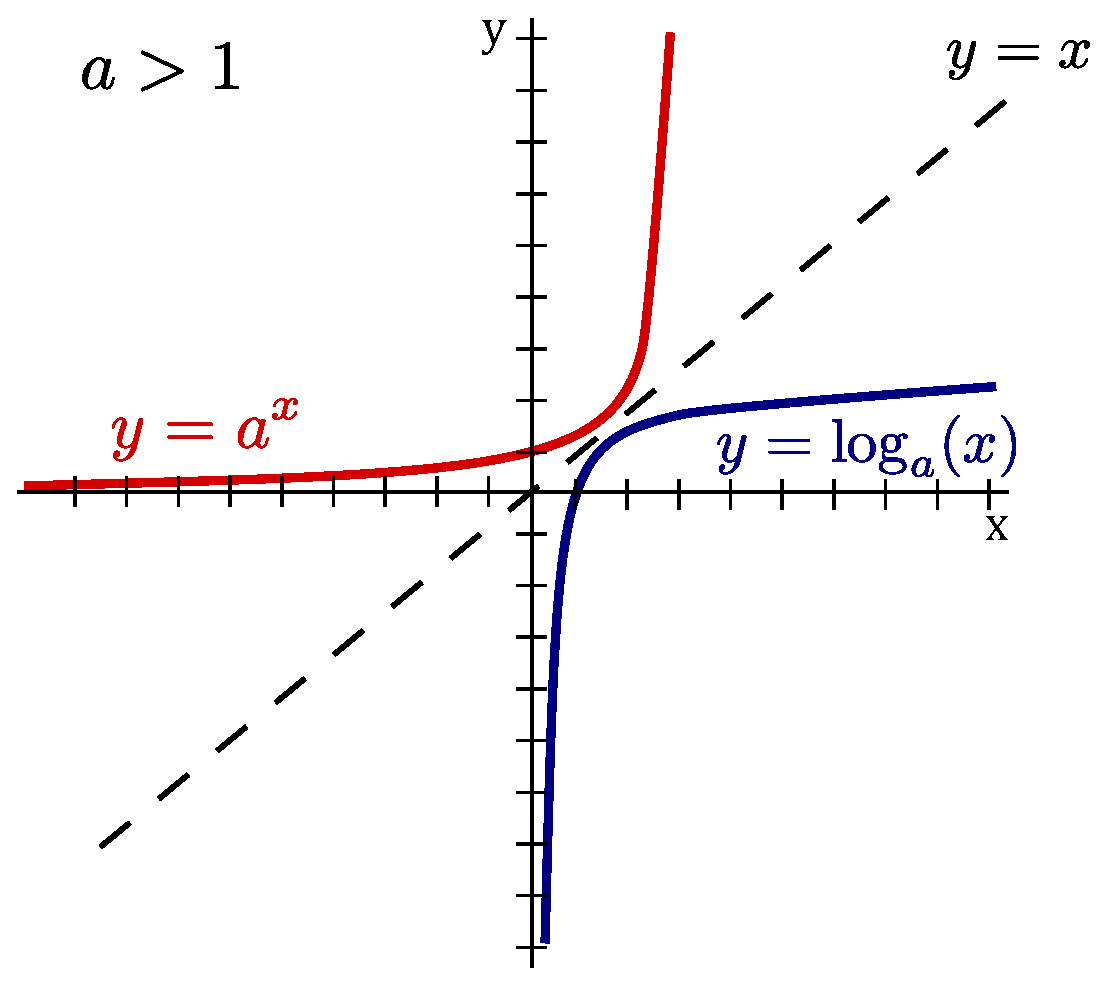
\includegraphics[width=3.0in]{images/log1}$$
Notice that every logarithm passes through the point $(1,0)$ in the same way that every exponential function passes through the point $(0,1)$.

Some properties of logarithms are as follows.

\begin{formulabox}[Logarithm Properties]
Let $A,B$ be positive numbers and $b>0$ ($b\neq1$) be a base.
\begin{itemize}
	\item $\ds{\log_b(AB)=\log_b A+\log_b B}$,
	\item $\ds{\log_b\left(\frac{A}{B}\right)=\log_b A-\log_b B}$,
	\item $\ds{\log_b(A^n)=n\log_b A}$, where $n$ is any real number.
\end{itemize}
\end{formulabox}

\begin{example}{Compute Lorarithms}{ComputeLorarithms}
To compute $\log_2(24)-\log_2(3)$ we can do the following:
$$\log_2(24)-\log_2(3)=\log_2\left(\frac{24}{3}\right)=\log_2(8)=3,$$
since $2^3=8$.
\end{example}

\subsection*{The Natural Logarithm}
As mentioned earlier for exponential functions, the number $e\approx 2.71828\ldots$ 
is the most convenient base to use in Calculus.
For this reason we give the logarithm with base $e$ a special name: \dfont{the natural logarithm}.
We also give it special notation:
$$\log_ex=\ln x.$$

You may pronounce $\ln$ as either: ``el - en'', ``lawn'', or refer to it as ``natural log''.
The above properties of logarithms also apply to the natural logarithm.
 
Often we need to turn a logarithm (in a different base) into a natural logarithm.
This gives rise to the \ifont{change of base formula}.

\begin{formulabox}[Change of Base Formula]
$$\log_ax=\frac{\ln x}{\ln a}.$$
\end{formulabox}

\begin{example}{Combine Logarithms}{CombineLogarithms}
Write $\ln A+2\ln B -\ln C$ as a single logarithm.
\end{example}

\begin{solution} 
Using properties of logarithms, we have,
$$\begin{array}{rcl}
\ln A+2\ln B -\ln C & = & \ln A + \ln B^2 - \ln C\\
~&=& \ln (AB^2) - \ln C\\
~&=& \ds{\ln\frac{AB^2}{C}}\\
\end{array}$$
\end{solution}

\begin{example}{Solve Exponential Equations using Logarithms}{SolveExponentialEquationsLogarithms}
If $e^{x+2}=6e^{2x}$, then solve for $x$.
\end{example}

\begin{solution} 
Taking the natural logarithm of both sides and noting the cancellation formulas (along with $\ln e=1$), we have:
$$\begin{array}{rcl}
e^{x+2} & = & 6e^{2x}\\
\\
\ln e^{x+2}&=& \ln (6e^{2x})\\
\\
x+2&=& \ln 6 + \ln e^{2x}\\
\\
x+2&=& \ln 6 + 2x\\
\\
x&=& 2-\ln 6\\
\end{array}$$
\end{solution}

\begin{example}{Solve Logarithm Equations using Exponentials}{SolveLogarithmEquationsExponentials}
If $\ln(2x-1)=2\ln(x)$, then solve for $x$.
\end{example}

\begin{solution} 
``Taking $e$'' of both sides and noting the cancellation formulas, we have:
$$\begin{array}{rcl}
e^{\ln(2x-1)} & = & e^{2\ln(x)}\\
\\
(2x-1) & = & e^{\ln(x^2)}\\
\\
2x-1 & = & x^2\\
\\
x^2-2x+1 & = & 0\\
\\
(x-1)^2 & = & 0\\
\end{array}$$
Therefore, the solution is $x=1$.
\end{solution}


%%%%%%%%%%%%%%%%%%%%%%%%%%%%%%%%%%%%%%%%%%%%
\Opensolutionfile{solutions}[ex]
\section*{Exercises for \ref{sec:Logarithms}}

\begin{enumialphparenastyle}

%%%%%%%%%%
\begin{ex}
Expand $\ds\log_{10} ((x+45)^7 (x-2))$.
\end{ex}

%%%%%%%%%%
\begin{ex}
Expand $\ds\log_2 {\frac{x^3}{3x-5 +(7/x)}}$.
\end{ex}

%%%%%%%%%%
\begin{ex}
Write $\ds \log_2 3x + 17 \log_2 (x-2) -
2\log_2 (x^2 + 4x + 1)$ as a single logarithm.
\end{ex}

%%%%%%%%%%
\begin{ex}
Solve $\ds \log_2 (1+ \sqrt{x} ) = 6$ for  $x$.
\end{ex}

%%%%%%%%%%
\begin{ex}
Solve $\ds 2^{x^2} = 8$ for $x$.
\end{ex}

%%%%%%%%%%
\begin{ex}
Solve $\ds \log_2 (\log_3 (x) ) = 1$ for $x$.
\end{ex}

\end{enumialphparenastyle}